\documentclass[ALICE,manyauthors]{cernphprep}

\usepackage[comma,square,numbers,sort&compress]{natbib}

\usepackage[T1]{fontenc} % if needed
\usepackage[utf8]{inputenc}
\usepackage[english]{babel}

\usepackage{amssymb}
\usepackage{hyperref}
\usepackage{lineno}
%\usepackage{subfig}
%\usepackage{subcaption}
\usepackage[amssymb]{SIunits}
\usepackage{booktabs}
\usepackage{multirow}
\usepackage{xcolor}
\usepackage{placeins}


% Custom commands to make typing the text easier
\newcommand{\pp}{\ensuremath{\mbox{p\kern-0.05em p}}}
\newcommand{\ppbar}{\ensuremath{\mathrm{p\kern-0.05em \bar{p}}}}
\newcommand{\pPb}{\ensuremath{\mbox{p--Pb}}}
\newcommand{\PbPb}{\ensuremath{\mbox{Pb--Pb}}}
\newcommand{\sqrtS}{\ensuremath{\sqrt{s}}}
\newcommand{\sqrtSnn}{\ensuremath{\sqrt{s_{\mathrm{NN}}}}}
\newcommand{\sqrtSE}[2][TeV]{\ensuremath{\sqrtS = #2~\mathrm{#1}}}
\newcommand{\sqrtSnnE}[2][TeV]{\ensuremath{\sqrtSnn = #2~\mathrm{#1}}}
\newcommand{\GeVc}{\ensuremath{\mathrm{GeV}\kern-0.05em/\kern-0.02em c}}
\newcommand{\gev}{\ensuremath{\mathrm{GeV}\kern-0.05em}}
\def\pt#1{\ensuremath{p_{\rm T#1}}} 
\def\jt#1{\ensuremath{j_{\rm T#1}}}
\def\vjt#1{\ensuremath{\vec{j}_{\rm T#1}}}
\def\kt#1{\ensuremath{k_{\rm T#1}}}
\newcommand{\xlong} {\ensuremath{x_{\parallel}}}
\def\mean#1{\left<#1\right>}
\def\rms#1{\ensuremath{\sqrt{\left<#1^2\right>}}}
\def\fig#1{Fig.~\ref{#1}}
\def\eq#1{Eq.~\eqref{#1}}
\DeclareUnicodeCharacter{00A0}{ }

\begin{document}

%%%%%%%%%%%%%%%  Title page %%%%%%%%%%%%%%%%%%%%%%%%
\begin{titlepage}
%
\PHyear{2018}
\PHnumber{XXX}      % required, will be obtained from PH
\PHdate{6 September}  % required, will be obtained from PH
%

%%% Put your own title + short title here:
\title{Jet fragmentation transverse momentum measurements correlations in $\sqrtSnnE{5.02}$ $\pPb$ collisions}
\ShortTitle{Jet fragmentation transverse momentum}   % appears on right page headers

%%% Do not change the next lines
\Collaboration{ALICE Collaboration\thanks{See Appendix~\ref{app:collab} for the list of collaboration members}}
\ShortAuthor{ALICE Collaboration} % appears on left page headers, do not change

\begin{abstract}
Jet fragmentation transverse momentum ($\jt{}$) distributions were studied using full jet reconstruction in proton-lead collisions at $\sqrtSnnE{5.02}$, measured with the ALICE experiment at the LHC. Jets from jet reconstruction with $ 40 < \pt{jet } <150$ were used for the calculation. The $\jt{}$ value was caculated for tracks inside an $R=0.4$ cone around the jet axis. The measured distributions show a clear narrow Gaussian component and a wide component described by an inverse gamma function. In previous studies the narrow component was related to hadronization and the wide component to the showering process. The width of the wide component increases with increasing jet transverse momentum, while the width of the narrow component has only a weak dependance on jet momentum. The results are compared to \textsc{Pythia} and Herwig simulations. Direct quantitative comparison to previous results from dihadron correlations is not possible, but qualitatively the results show similar trends.
\end{abstract}
\end{titlepage}
\setcounter{page}{2}

%%%%% Body of the article
% !TEX root = jetjtPaperPreview.tex
\linenumbers

%% main text
\section{Introduction}
\label{sec:introduction}
Jets are collimated sprays of hadrons originating from the fragmentation of hard partons produced in high-energy particle collisions. Studying the jet fragmentation can give insight into Quantum Chromodynamics (QCD)~\cite{gross1973ultraviolet, politzer1973reliable, gross1973asymptotically, gross1974asymptotically, georgi1974electroproduction}, phenomena, such as angular ordering~\cite{basicsofpqcd} and hadronisation. In this work the fragmentation of partons is studied using the jet fragmentation transverse momentum, $\jt{}$, which is the perpendicular component of the momentum with respect to the momentum vector of the initial hard parton.

Previously, $\jt{}$ has been studied using two-particle correlations by the CCOR collaboration at ISR in $\pp$ collisions at center-of-mass energy $\sqrtS = 31,\;45$ and $63~\mathrm{GeV}$~\cite{firstjtmeasurement} and the PHENIX collaboration at RHIC in $\pp$ collisions at $\sqrtSE[GeV]{200}$~\cite{PHENIXjets} and d--Au collisions at center-of-mass energy per nucleon pair $\sqrtSnnE[GeV]{200}$~\cite{phenixJtPAu}. 
Jet measurements to study $\jt{}$ have been done by the CDF collaboration at the Tevatron in $\ppbar$ collisions at $\sqrtSE{1.96}$~\cite{cdfpaper} and the ATLAS collaboration at the LHC in $\PbPb$ collisions at $\sqrtSnnE{2.76}$~\cite{atlaksenJetit}.
%Recently $\jt{}$ with two-particle correlations was studied at ALICE~\cite{ALICEjt}.
Jet production in QCD can be thought of as two separate stages~\cite{eventGenerators}. After being produced in the hard scattering, partons reduce their high virtuality through emitting gluons. Since the transverse momentum scale ($Q^{2}$) is large during the showering, perturbative QCD calculations can be applied. When $Q^{2}$ becomes of the order of $\Lambda_{\mathrm{QCD}}$, partons hadronize into final-state particles through a non-perturbative process. 

In practice these two stages happen at least in part simultaneously. %{\color{red} [Showering time vs hadronisation time ]}
Thus it is not a priori clear that the effect of them can be separated. Recently ALICE classified the two distinct components using two-particle correlations~\cite{ALICEjt}.The goal of this study is to see if similar identification of components is possible in a jet reconstruction-based study. 

As non-perturbative processes these are hard to calculate from first principles. Instead Monte Carlo generators such as \textsc{Pythia}~\cite{introPythia81} and Herwig~\cite{Herwig7releaseNote} are used to produce a theoretical background. One approach based on perturbative QCD (pQCD) is the Next-to-Modified Leading Log Approximation (NMLLA)~\cite{nmlla}. This approach implements local parton hadron duality (LPHD) instead of any more sophisticated hadronisation model.

These two MC generators handle both the showering process and hadronisation differently. Pythia uses the Lund string model~\cite{lundString} to perform the hadronisation stage. Herwig uses a cluster model for the hadronisation. Pythia 6 has $\pt{}$ ordered showers while Pythia 8 has rapidity ordered showers. Herwig simulates parton showers using the coherent branching algorithm of~\cite{Gieseke:2003rz}. This algorithm has angular ordering as a central feature. In \textsc{Pythia} 8 angular ordering is built in, while in \textsc{Pythia} 6 it can be turned on or off.

Jets also are used as an important probe for the study of the deconfined phase of strongly interacting QCD matter, the quark-gluon plasma (QGP) that is created in high energy collisions of heavy nuclei.
There have been many experimental evidences of jet energy loss, such as the suppression of inclusive hadron spectra at high transverse momentum, the modification of back-to-back hadron-hadron and direct photon-hadron correlations, and the modification of reconstructed jet spectra and jet substructure, as compared to the expectations from elementary proton-proton collisions.

Jet quenching in heavy-ion collisions evolves multi-scale problems~\cite{Kurkela:2014tla,Tachibana:2018yae}. The elementary scattering and the subsequent branching process down to non-perturbative scales are dominated by hard scales in the vacuum as well as in the medium. Soft scales, of the order of the temperature of the medium, characterise the interactions of soft partons produced in the shower with the QGP. Soft scales also rule hadronisation, which is expected to take place in vacuum for sufficiently energetic probes. Understanding the contributions from the different processes to the jet shower evolution in medium and their scale dependence is crucial to to constrain the dynamics of jet energy loss in the expending medium, the role of colour coherence~\cite{CasalderreySolana:2012ef}, and fundamental medium properties like temperature dependent transport coefficient~\cite{DEramo:2012uzl,Ayala:2016pvm}.

The observed strong collective behavior suggests that the QGP is created in high multiplicity pp and pA collisions~\cite{Abelev:2012ola,Aad:2012gla,Chatrchyan:2013nka,Khachatryan:2010gv,Khachatryan:2016txc,Aidala:2016vgl}.  Jet production could be modified even if the collision system is small~\cite{Zhang:2013oca,Park:2016jap,TYWONIUK201485}, though no clear consensus on the magnitude of the quenching has been made. There had been no evidence of jet quenching in minimum bias collisions~\cite{Khachatryan:2016odn,ALICEjt}, i.e. averaged over all events.  However, in these small systems, the selection of event class based on multiplicity has strong autocorrelations between the nature of the nucleon-nucleon collisions and the hard process itself. This makes the interpretation of experimental observables complicated~\cite{Adam:2014qja, Adam:2016jfp,Nagle:2018nvi} because the measurements are limited on the cross section of high-\pt{} hadrons and jets. 
 
% only done in minbias events and there are biases 

In this paper, the $\jt{}$ distributions are studied by reconstructing the jets with jet algorithms~\cite{antikt} in $\sqrtSnnE{5.02}$ $\pPb$ minimum bias and high multiplicity collisions. The advantage of jet reconstruction is that it should give a better estimate of the initial hadron momentum when compared to using two-particle correlations. Additionally the results are not smeared by the splitting of the leading hadron as was the case in the correlation study. The disadvantage is that the jet reconstruction limits the study to a small cone around the jet axis. Additionally the kinematics of produced jets are different. In dihadron analysis, the results are done in $\pt{trigger}$ bins, which favours harder jets (leading track carries a large fraction of the momentum). When looking at $\pt{jet}$ bins softer jets are favored.


This paper is structured as follows. The event and track selection together with the used data samples are described in Sec.~\ref{sec:experimentaldetails}. The analysis details are discussed in Sec.~\ref{sec:methods}, followed by the systematic uncertainty analysis in Sec.~\ref{sec:systematicerrors}. The obtained results are shown in Sec.~\ref{sec:results} and the observations are summarized in Sec.~\ref{sec:conclusions}.


\section{Experimental setup and data samples}
\label{sec:experimentaldetails}
The $\sqrtSnnE{5.02}$ $\pPb$ ($1.3 \cdot 10^{8}$ events, $\mathcal{L}_{\mathrm{int}} = \unit[620]{nb^{-1}}$) collisions were recorded in 2013 by the ALICE detector~\cite{aliceDetector}. The details of the performance of the ALICE detector during LHC Run~1 (2009-2013) are presented in Ref.~\cite{alicePerformance}.

The analysis uses charged tracks that are reconstructed with the Inner Tracking System (ITS)~\cite{aliceITS} and the Time Projection Chamber (TPC)~\cite{aliceTPC}. These detectors are located inside the large solenoidal magnet, that provides a homogeneous magnetic field of \unit[0.5]{T}. Tracks within a pseudorapidity range $|\eta| < 0.9$ over the full azimuth can be reconstructed. The ITS is made up of the innermost Silicon Pixel Detector (SPD), the Silicon Drift Detector (SDD) and the outermost Silicon Strip Detector (SSD). Each of these consists of two layers. The TPC is a cylinder filled with gas. Gas is ionised along the path of charged particles. Liberated electrons drift towards the end plates of the cylinder where they are detected. Combining the information from the ITS and the TPC provides a resolution ranging from $1$ to $10\,\%$ for charged particles with momenta from $0.15$ to $\unit[100]{\GeVc}$. For tracks without the ITS information, the momentum resolution is comparable to that of ITS+TPC tracks below transverse momentum $\pt{} = \unit[10]{\GeVc}$, but for higher momenta the resolution reaches $20\,\%$ at $\pt{} = \unit[50]{\GeVc}$~\cite{alicePerformance,aliceBackgroundFluctuation}. 

Neutral particles used in jet reconstruction are reconstructed by the Electromagnetic Calorimeter (EMCAL)~\cite{Cortese:2008zza}. The EMCAL covers an area with a range of $|\eta| < 0.7$  in pseudorapidity and $ 100 \deg $ in azimuth. EMCAL is complimented with the Dijet Calorimeter (DCal)~\cite{DCAL} and Photon Spectrometer (PHOS)~\cite{PHOS} that are situated opposite of the EMCAL in azimuth. PHOS covers 70 degrees in azimuth and $\left| \eta \right| < 0.12$. The DCal is technologically identical to EMCal. The DCal coverage spans over 67 degrees in azimuth, but in pseudorapidity the mid region is occupied by the PHOS. In between PHOS and DCal active volumes, there is a gap of 10 cm. DCal is fully back-to-back with EMCal.

The combination of charged tracks with  $\pt{} > \unit[0.15]{\GeVc}$ and neutral particles with $\pt{} > \unit[0.30]{\GeVc}$ is used to construct jets. 

The V0 detector~\cite{forwarddetectorsTdr} provides the information for event triggering. The V0 detector consists of two scintillator hodoscopes that are located on either side of the interaction point along the beam direction. It covers the pseudorapidity region $-3.7 < \eta < -1.7$ (V0C) and $2.8 < \eta < 5.1$ (V0A). For the 2013 $\pPb$ collisions events are required to have signals in both V0A and V0C. This condition is used later offline to reduce the contamination of the data sample from beam-gas events by using the timing difference of the signal between the two stations~\cite{alicePerformance}.

%For the 2010 $\pp$ collisions, the minimum bias (MB) triggered events are required to have at least one hit from a charged particle traversing the SPD or either side of the V0. 
%The pseudorapidity coverage of the SPD is $|\eta| < 2$ in the first layer and $|\eta| < 1.5$ in the second layer. %Combining this with the acceptance of the V0, the particles are detected in the range $-3.7 < \eta < 5.1$. The minimum %bias trigger definition 

EMCAL is also used to provide the jet trigger used in triggered datasets. EMCAL can be used to trigger on single shower deposits or energy deposits integrated over a larger area. Latter case is used for jet triggers. The EMCAL trigger definition in the 2013 $\pPb$ collisions requires an energy deposit of either 10 \gev for the low threshold trigger or 20 \gev for the high threshold trigger in a $32\times32$ patch size.

%For the $\pp$ collisions, similar track cuts as in Ref.~\cite{ALICE:2011ac} are used: at least two hits in the ITS are required, one of which needs to be in the three innermost layers, and 70 hits out of 159 are required in the TPC. In addition, the distance of the closest approach (DCA) of the track to the primary vertex is required to be smaller than $\unit{2}{cm}$ in the beam direction. In the transverse direction, a $\pt{}$ dependent cut DCA $< \unit{0.0105}{cm} + \unit{0.035}{cm} \cdot \pt{}^{-1.1}$ is used, where $\pt{}$ is measured in units of $\GeVc$. These track cuts are tuned to minimize the contamination from secondary particles.

%In $\pPb$ collisions the tracks are selected following the hybrid approach~\cite{hybridExplanation}. In this method tracks with at least one hit in the SPD and at least two hits in the whole ITS are always accepted. In addition, tracks with fewer than two hits in the ITS or no hits in the SPD are accepted, but only if an additional vertex constraint is fulfilled. In addition, the distance of the closest approach (DCA) of the track to the primary vertex is required to be smaller than $\unit{3.2}{cm}$ in the beam direction and smaller than $\unit{2.4}{cm}$ in the transverse direction. This approach is not affected by dead regions ins SPD. Thus it produces an azimuthal angle ($\varphi$) distribution that is as uniform as possible. The momentum resolutions of the two classes of particles are comparable up to $\pt{} \approx 10\;\GeVc$, but after that, tracks without ITS requirements have a worse resolution~\cite{alicePerformance,aliceBackgroundFluctuation}.
In $\pPb$ collisions the tracks are selected following the hybrid approach~\cite{hybridExplanation} which ensures a uniform distribution of tracks as a function of azimuthal angle ($\varphi$). The momentum resolutions of the two classes of particles are comparable up to $\pt{} \approx 10\;\GeVc$, but after that, tracks without ITS requirements have a worse resolution~\cite{alicePerformance,aliceBackgroundFluctuation}.

\section{Analysis method}
\label{sec:methods}

The analysis is performed by analysing jet constituents. In each collision event, the jets are reconstructed using FastJet~\cite{fastjet} with the anti-$\kt{}$ algorithm~\cite{antikt}. Jets for R=0.4 are selected in $\left| \eta \right| < 0.25 $ to satisfy the fiducial acceptance of the EMCal.In jet reconstruction both charged tracks with $\pt{}>\unit[0.15]{\GeVc}$ and neutral cluster with $\pt{}>\unit[0.30]{\GeVc}$ are considered. In the analysis, results are presented in terms of the jet transverse momentum $\pt{jet}$.

The jet fragmentation transverse momentum, $\jt{}$, is defined as the component of the constituent particle momentum, $\vec{p}_{\mathrm{a}}$, transverse to the jet momentum, $\vec{p}_{\mathrm{jet}}$. The resulting $\vjt{}$ is illustrated in~\fig{fig:jtdefinition}. The length of the $\vjt{}$ vector is
  \begin{equation}
    \jt{} = \frac{|\vec{p}_{\mathrm{jet}} \times \vec{p}_{\mathrm{track}}|}{|\vec{p}_{\mathrm{jet}}|} \,.
  \label{eq:jtdefinition}
  \end{equation}

It is commonly interpreted as a transverse kick with respect to the initial hard parton momentum that is given to a fragmenting particle during the fragmentation process, which is a measure of the momentum spread of the jet fragments~\cite{}. 

The reconstructed jet axis is used for $\jt{}$ reference. Any charged track within a fixed cone with radius $R$ is taken as a jet constituent, as opposed to using the constituent list provided by the jet algorithm. Anti-$\kt{}$ produces jets that are very circular in shape. Thus this doesn't change the constituent list considerably. Neutral tracks are used only in jet reconstruction.
 
The resulting $\jt{}$ distributions are corrected for the detector inefficiency using the unfolding method. The response matrix for the unfolding is obtained from a \textsc{Pythia}~\cite{introPythia81} simulation.
 
   \begin{figure}
    \begin{center}
      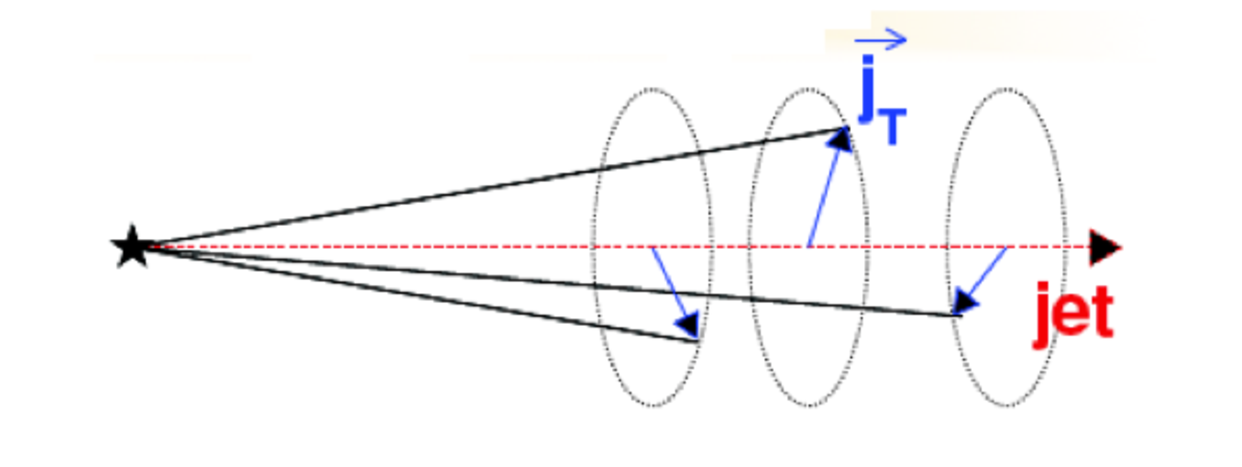
\includegraphics[width = 0.60\textwidth]{figures/jt_def}
    \end{center}
    \caption{Illustration of $\vjt{}$. The jet fragmentation transverse momentum, $\vjt{}$, is defined as the transverse momentum component of the track momentum, $\vec{p}_{\mathrm{track}}$, with respect to the jet momentum, $\vec{p}_{\mathrm{jet}}$.}
    \label{fig:jtdefinition}
  \end{figure}
 
The underlying event is estimated by looking at an imaginary jet cone perpendicular to the observed jet axis ($\frac{\pi}{2}$ Rotation in $\phi$). $\jt{}$ is calculated for any tracks found within this cone. The vector sum of the individual track momentum and the imaginary jet axis is used as reference for $\jt{}$. The background obtained in this manner is subtracted from the unfolded inclusive $\jt{}$ distribution, which gives the resulting signal distribution. To make sure there is no jet contribution in the background, any events with jets inside the perpendicular cone are not used for background estimation.

 

The resulting signal distribution are fitted with a 2 component function shown in Eq.~\ref{eq:fit}. Gaussian distribution is used for low $\jt{}$ and an inverse gamma function is used for high $\jt{}$. The gaussian is taken to have the center at $\jt{} = 0$. In total this gives 5 parameters.

\begin{equation}
\frac{1}{N_{\mathrm{jets}}}\frac{\mathrm{d}N}{\jt{} \mathrm{d}\jt{}} = \frac{B_2}{B_1\sqrt{2\pi}}e^{-\frac{\jt{}^2}{2B_1^2}}+\frac{B_3B_5^{B_4}}{\Gamma\left(B_4\right)}\frac{e^{-\frac{B_5}{\jt{}}}}{\jt{}^{B_4+1}}
\label{eq:fit}
\end{equation}

To achieve stable results the fitting is performed in two steps. First each component is fitted separately. Gaussian component is fitted to the low end in $\jt{}$. Inverse gamma component is fitted to $\jt{}$ above $\unit[1]{\GeVc}$. After getting the results from the individual fits they are combined into a single function with initial values from the individual results and an additional fit is performed. The result from fitting only 
the gaussian component to the entire distribution is approximately the same as the gaussian component in the two-component model.

After getting the fit function $\sqrt{\left<\jt{}^2\right>}$ (RMS) and yield values are  extracted separately from each component. The narrow component RMS is

$$\sqrt{\left<\jt{}^2\right>}=\sqrt{2}B_1,$$

and the wide component RMS value is calculated as 

$$\sqrt{\left<\jt{}^2\right>}=\frac{B_5}{\sqrt{\left(B_4-2\right)\left(B_4-3\right)}},$$

where it is required that $B_4 > 3$.

\section{Systematic uncertainties}
\label{sec:systematicerrors}
The systematic uncertainties in this analysis come from the background estimation, the unfolding procedure and the cuts used to select the tracks. Tracking uncertainties are estimated from variations of the track selection cuts defined in Sec.~\ref{sec:experimentaldetails}. The resulting variations in RMS are shown in Table \ref{tab:systematics}. The uncertainties from unfolding and background subtraction are of the same magnitude. 

The systematics in background estimation were studied using an alternative method to extract the background, mainly the random background method. The resulting uncertainty is below 5\% for the wide component RMS and below 9\% for the narrow component RMS. 

The systematic uncertainty that arises from the unfolding procedure is estimated by performing the unfolding with two separate methods. Data corrected by the iterative unfolding method are used as the results and the SVD unfolding method is employed to estimate the uncertainty. In a \textsc{Pythia} closure test the true distribution was in general found to be between the unfolded distributions from the iterative and SVD method. The difference between the methods when unfolding data should give a reasonable estimate of the unfolding uncertainty. The resulting uncertainty is below 8\% for both wide and narrow component RMS.

The different source of the systematic uncertainty are considered as uncorrelated and the values of each source are summed in quadrature. The resulting uncertainty is 9 \% for the wide component RMS and 12 \% for the narrow component RMS. 

\begin{table}[htb]
\centering
\caption{Summary of systematic errors}
\label{tab:systematics}
\begin{tabular}{ l | c | r }
  Systematic & Wide RMS & Narrow RMS \\
    \hline			
  Background & 5 \% & 9 \% \\
  Unfolding & 8 \% & 8 \% \\
  Tracking & ? \% & ? \% \\
  Total & 9 \% & 12\% \\
  \hline
  \end{tabular}
  \end{table}

There is no tracking and no unfolding uncertainty in the Monte Carlo simulations. 


%
%The systematic uncertainties considered for this analysis arise from the background determination, the signal fitting procedure and the cuts used to select the tracks. The uncertainties related to the tracking are estimated from variations of the track selection cuts defined in Section~\ref{sec:experimentaldetails}. The resulting variations of the RMS and yield are below 3~\% in most cases, but effects up to 17~\% are observed for the yield of the wide component. The tracking efficiency contributes to the uncertainty of the yields only. This uncertainty is estimated from the difference between data and simulation in the TPC-ITS track matching efficiency as is previously done in Refs.~\cite{spectrumReferencePp} and~\cite{spectrumReferencepPb}.  For $\pp$ this uncertainty is 5~\% and for $\pPb$ 4~\%. The effect where the subleading track is reconstructed as a leading track, because of detector inefficiencies, was studied using simulations and found to be negligible due to steep slope of the trigger spectrum.
%


\section{Results}
\label{sec:results}

Distributions of $\jt{}$ after unfolding and background subtraction are shown in Fig. \ref{fig:jtdist}. The yield at low $\jt{}$ stays constant with increasing $\pt{jet}$. At high $\jt{}$ the yield increases and the distributions become wider. In part this is due to kinematical limits. Within a fixed cone the maximum $\jt{}$ depends on the track momentum. 

$$\jt{max} \approx R \cdot \pt{track}$$

With increasing jet $\pt{}$ the possible track momenta also increase.

The distributions are fitted using a two component fit. An example of the fitted distribution is shown in Fig. \ref{fig:jtfit}. The $\jt{}$ distributions are well described by the two component model fit. 

\begin{figure}[htb]
\begin{center}
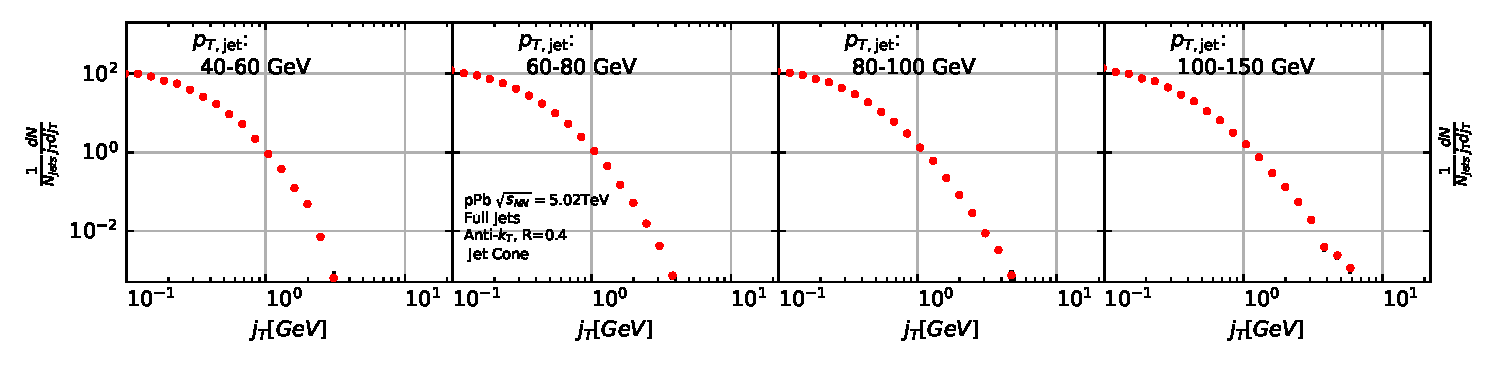
\includegraphics[width=0.95\textwidth]{figures/results/MixedFullJetsR04JetConeJtSignalPtFrom4To8.pdf}
%python Python/DrawSignal.py CF_pPb_legotrain/legotrain_CF_pPb_1839_20180613_LHC13bcde.root 0 4 8
\caption{$\jt{}$ distributions in different jet $\pt{}$ bins.}
\label{fig:jtdist}
\end{center}
\end{figure}

%\begin{figure}[htb]
%\begin{center}
%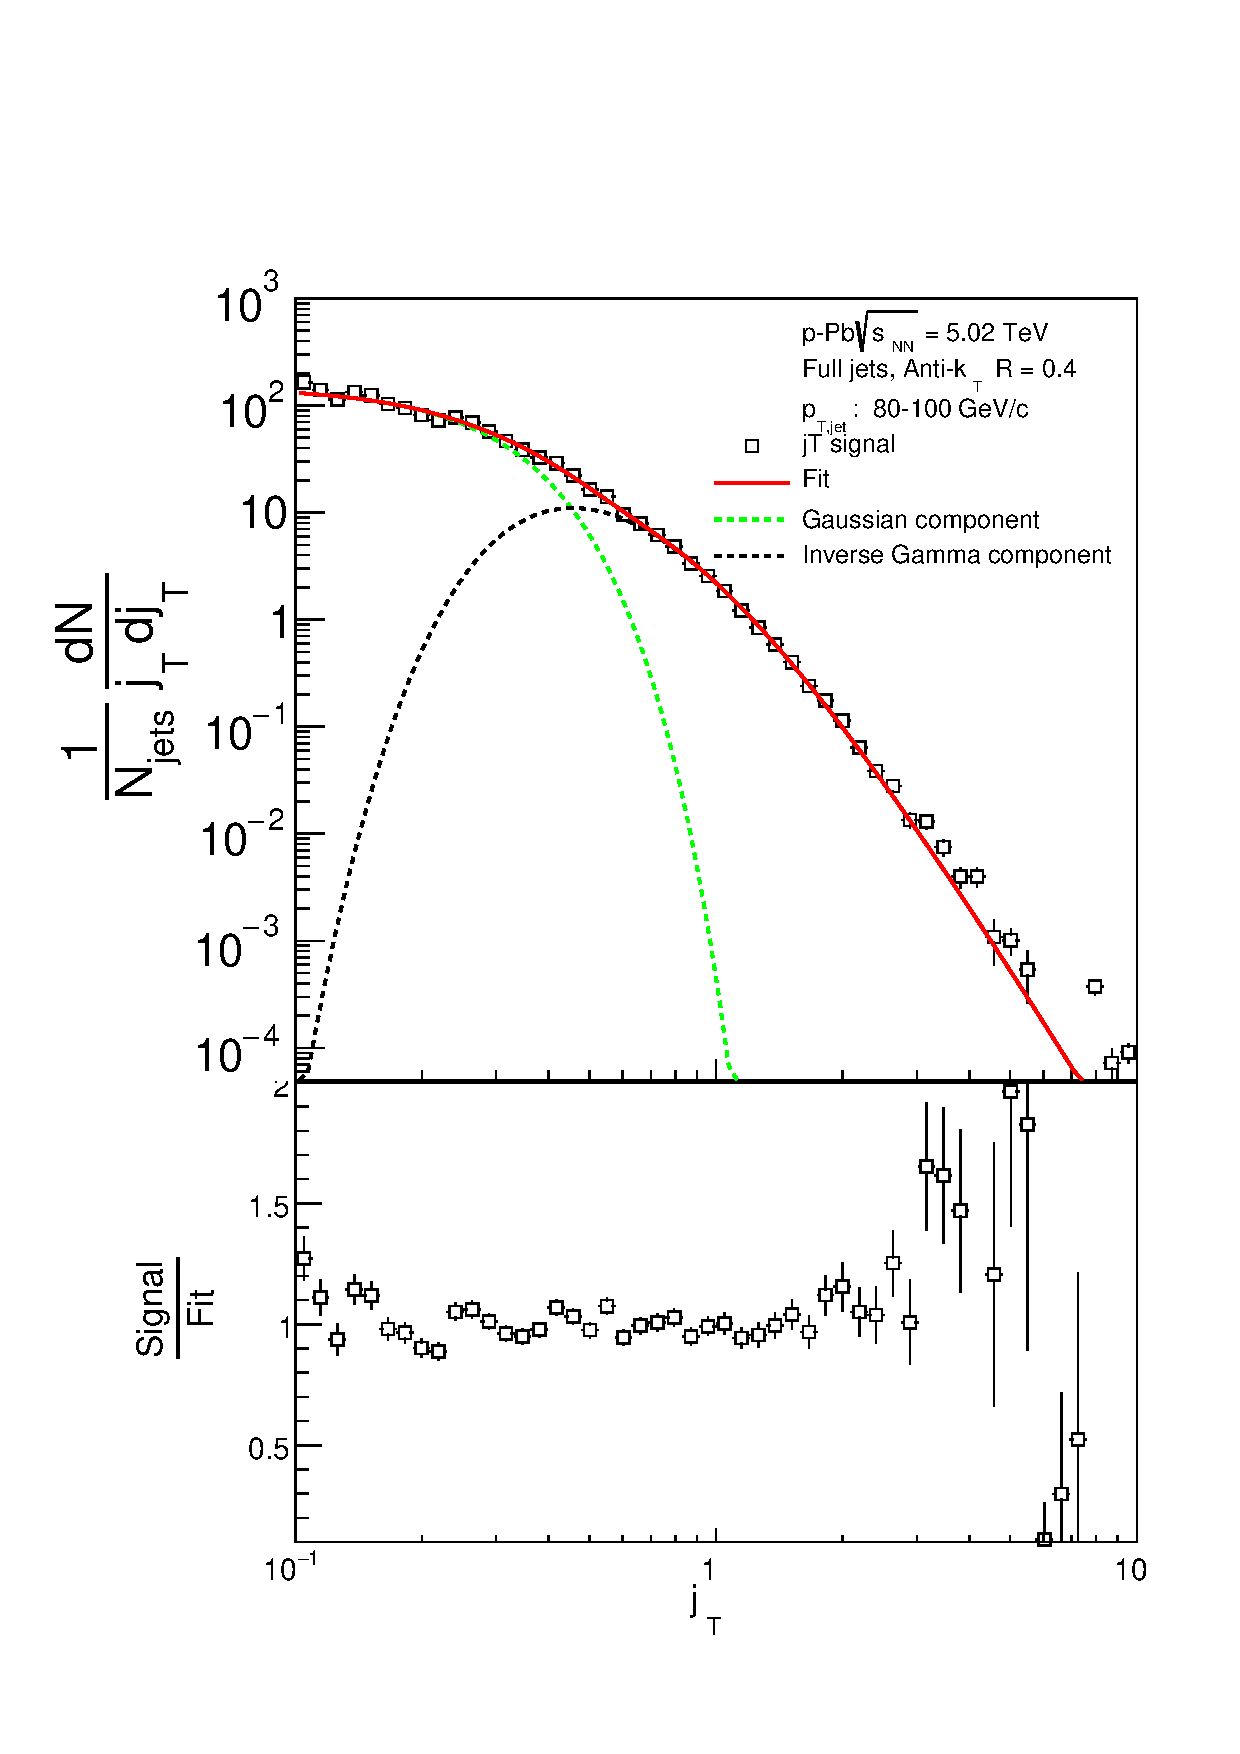
\includegraphics[width=0.5\textwidth]{figures/results/JetConejTSignalFitNFin00JetPt06perconeBgBayes.pdf}
%%python Python/DrawSignal.py CF_pPb_legotrain/legotrain_CF_pPb_1839_20180613_LHC13bcde.root 0 4 8
%\caption{$\jt{}$ distributions in different jet $\pt{}$ bins.}
%\label{fig:jtfit}
%\end{center}
%\end{figure}

The per jet yields and widths of the $\jt{}$ distributions are determined as a function of the transverse momentum of jet. The results are obtained from the area and RMS of the fits to the narrow and wide components of the $\jt{}$ distribution. The RMS $\left(\rms{\jt{}}\,\right)$ values for the narrow component are shown in \fig{fig:rmsgamma} with comparison to Monte Carlo simulations. 

There is clear separation in the width of the wide and narrow components of the $\jt{}$ distributions. The RMS of the wide component is 3-4 times larger than the narrow component RMS. The wide component is assumed to correspond to the fragmentation part of jet formation while the narrow component is linked with the hadronisation phase.

The wide component RMS shows an increasing trend with increasing $\pt{jet}$, while the narrow component RMS stays roughly constant. Both of these trends are qualitatively consistent with the results seen in dihadron $\jt{}$ analysis~\cite{ALICEjt}

\textsc{Pythia} describes well the RMS values in both the narrow and wide components. Herwig...({\color{red} insert observations from Herwgig}) \textsc{Pythia} uses the Lund string model for hadronisation while Herwig uses a cluster model. It seems ... 

%\begin{figure}[htb]
%\begin{center}
%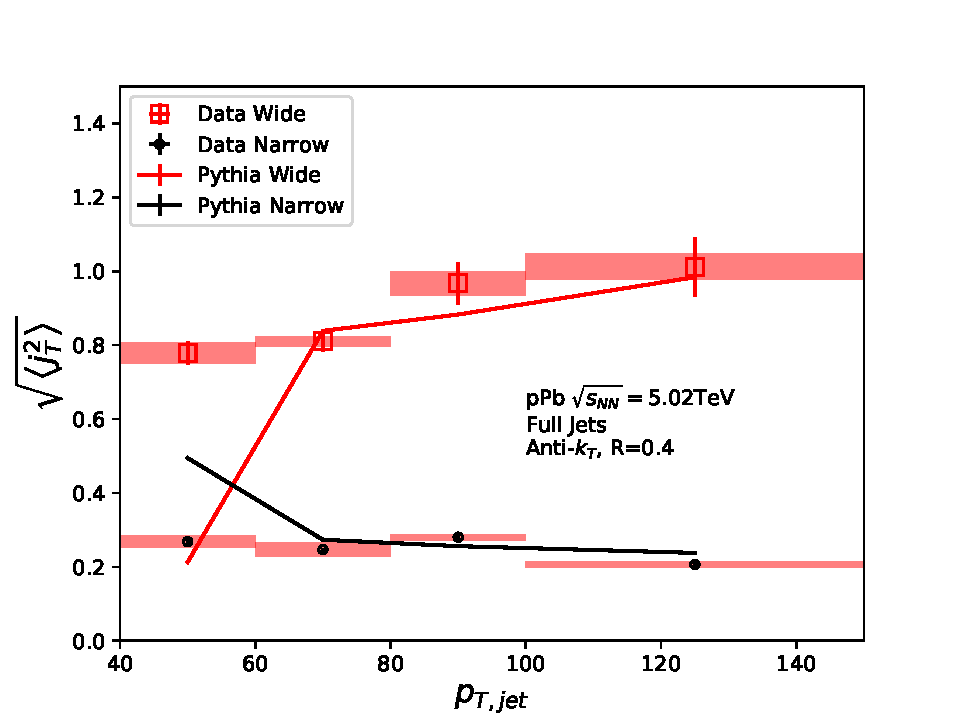
\includegraphics[width=0.55\textwidth]{figures/results/RMSWithSystematics_Pythia}
%\caption{RMS and yield values extracted from the fits for the gaussian (narrow) and inverse gamma (wide) components}
%\label{fig:rmsgamma}
%\end{center}
%\end{figure}

\begin{figure}[htp]
\centering
\subfigure[$\jt{}$ distribution with two component fitting]{\label{fig:jtfit} 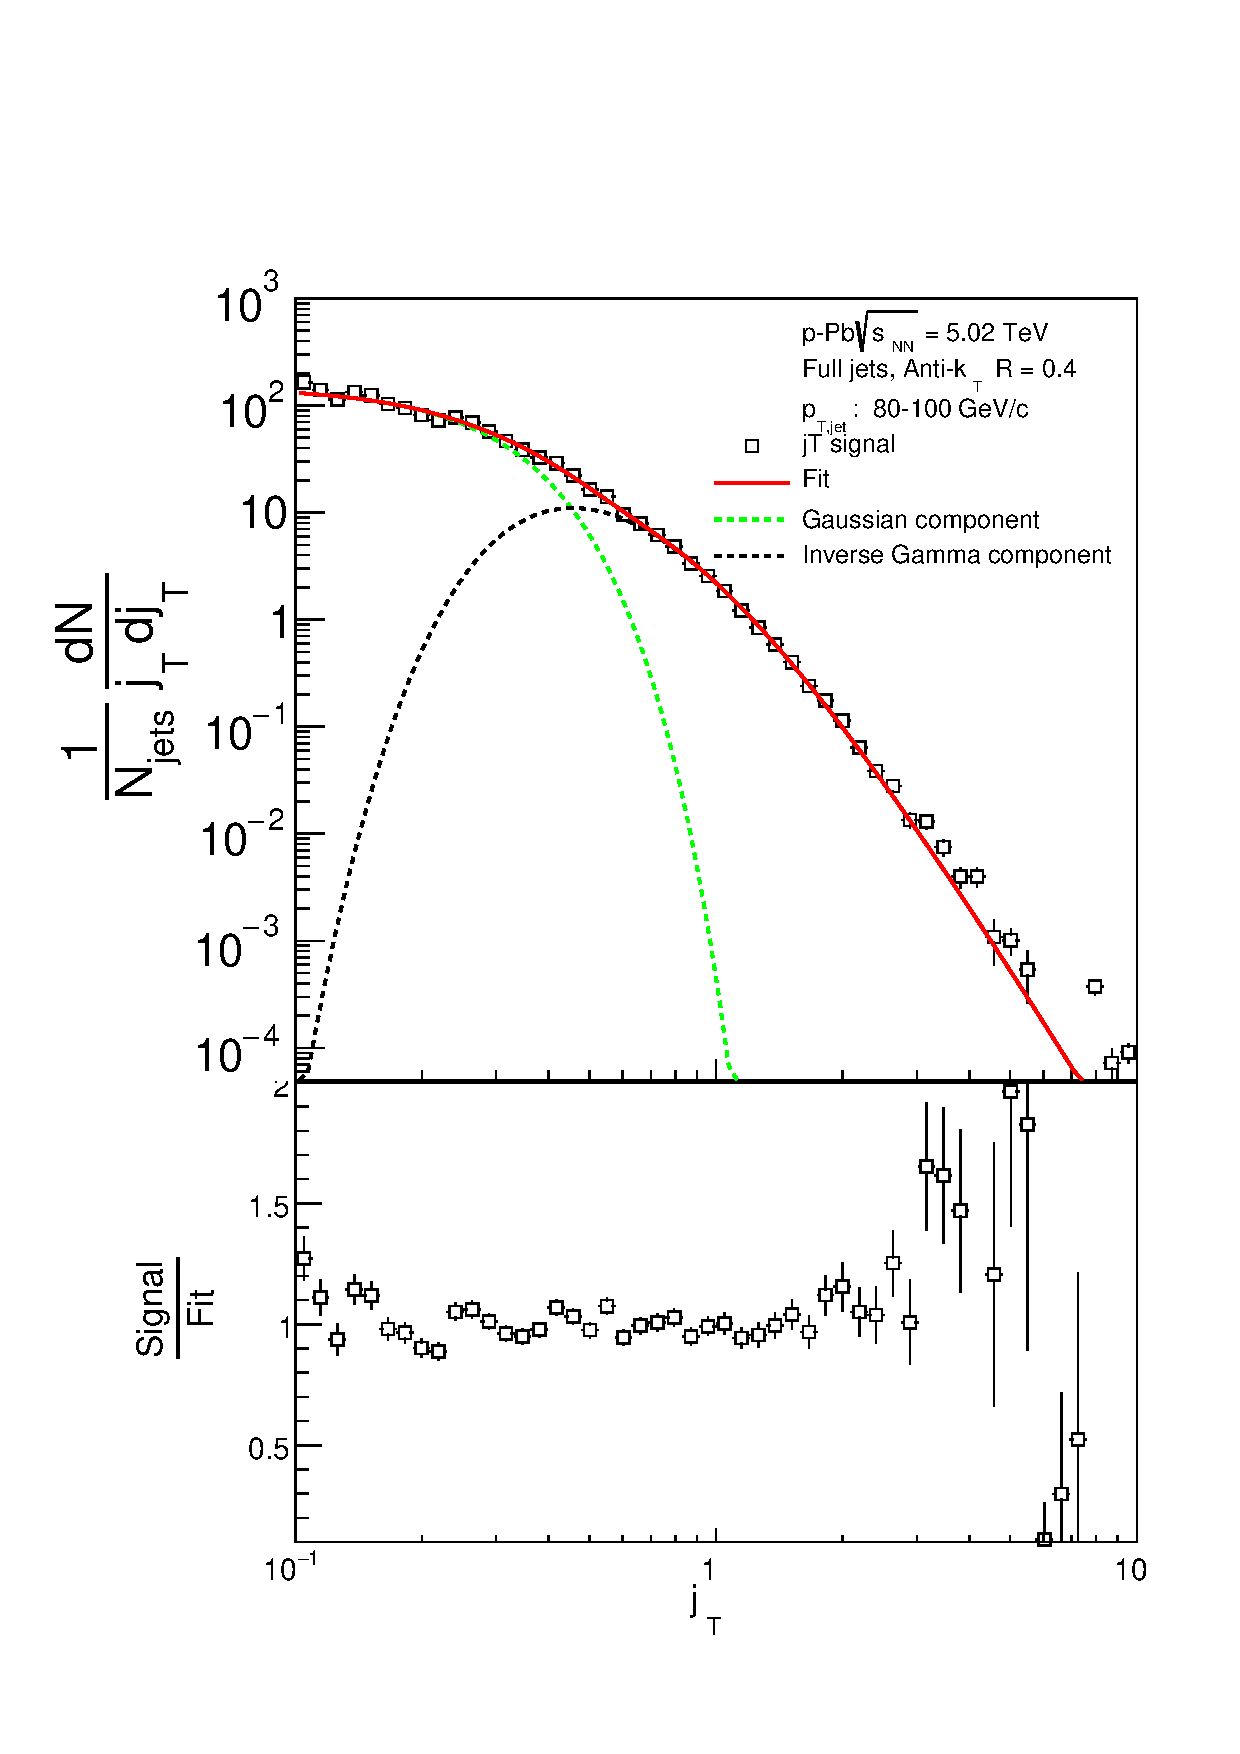
\includegraphics[width = 0.49\textwidth]{figures/results/JetConejTSignalFitNFin00JetPt06perconeBgBayes.pdf}}
\subfigure[RMS and yield values extracted from the fits for the gaussian (narrow) and inverse gamma (wide) components]{\label{fig:rmsgamma} 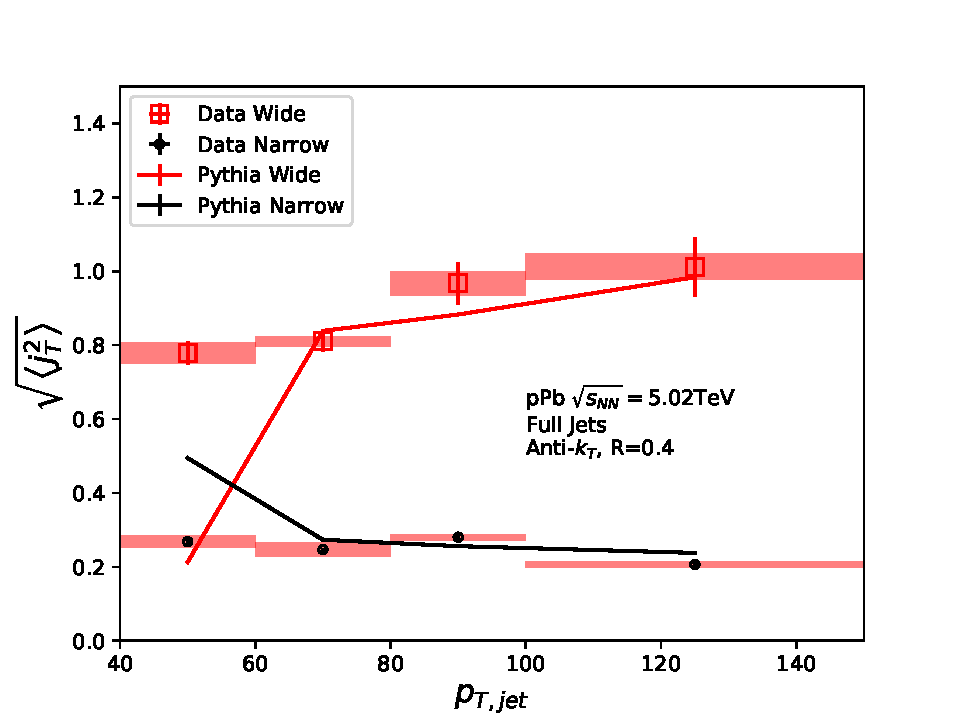
\includegraphics[width = 0.49\textwidth]{figures/results/RMSWithSystematics_Pythia}}
\caption{}
\label{fig:results}
\end{figure}


\FloatBarrier

\subsection{Discussion}
\begin{figure}[htb]
\centering
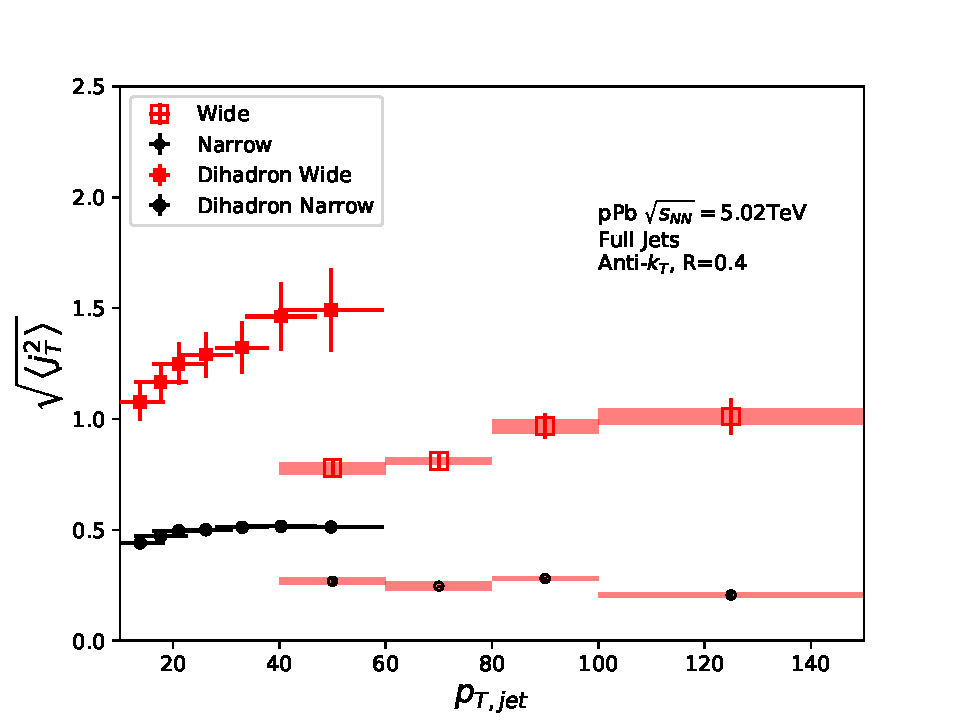
\includegraphics[width=0.55\textwidth]{figures/results/RMSWithSystematics_DihadronJetPt}
%\subfigure{ 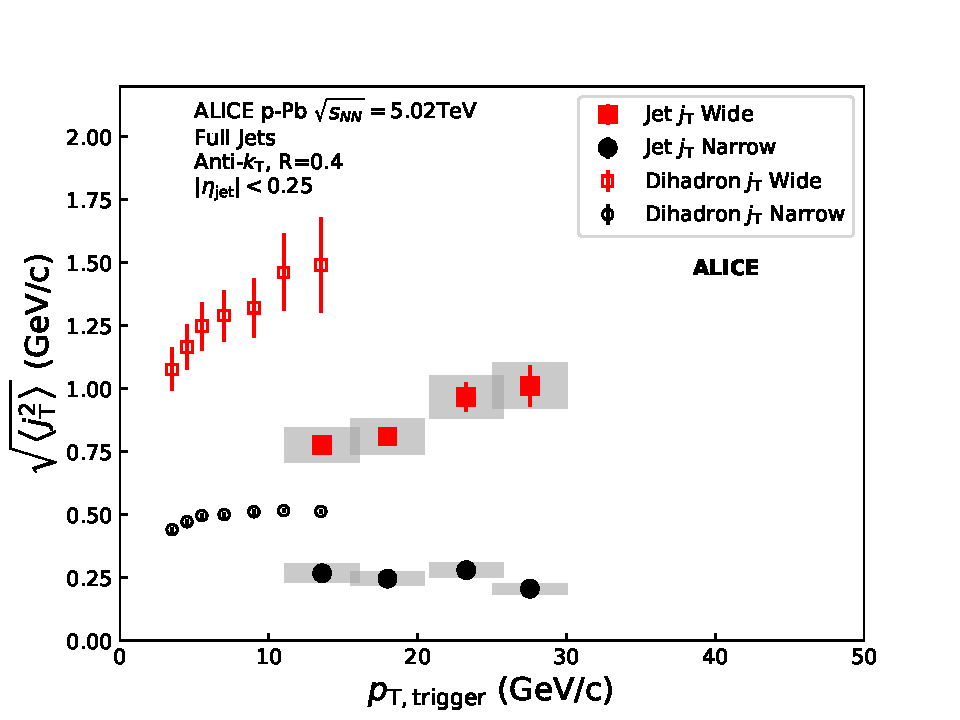
\includegraphics[width = 0.42\textwidth]{figures/results/RMSWithSystematics_DihadronTriggerPt}}
%\subfigure{ 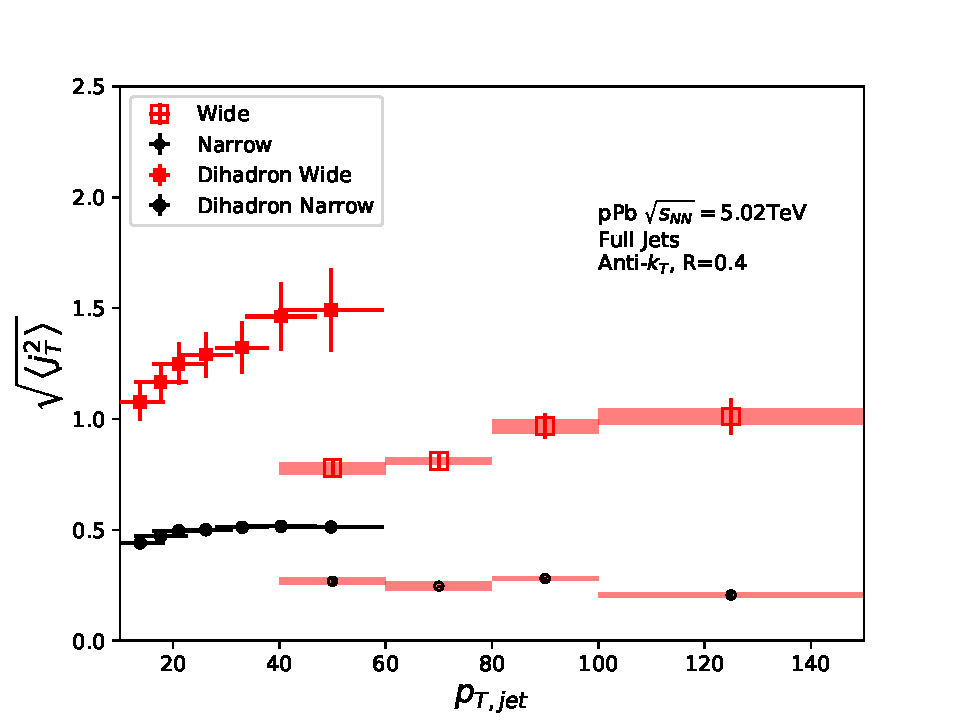
\includegraphics[width = 0.42\textwidth]{figures/results/RMSWithSystematics_DihadronJetPt}}
\caption{Comparison of results with dihadron $\jt{}$ results. Dihadron trigger $\pt{}$ bins are converted to jet $\pt{}$  bins  using observed mean  $\pt{jet}$ values in $\pt{trigger}$ bins. Dihadron results are for $0.2 < x_{||} < 0.4$ }
\label{fig:DihadronComparison}
\end{figure}

Comparison to $\jt{}$ results from dihadron analysis ~\cite{ALICEjt} is shown in Fig. \ref{fig:DihadronComparison}. Trigger $\pt{}$ bins used in dihadron analysis are converted to jet $\pt{}$ bins using observed average jet $\pt{}$ values in leading track momentum bins. Simlarly jet $\pt{}$ bins are converted to $\pt{trigger}$ bins using average leading track $\pt{}$ values in $\pt{jet}$ bins.

The trends are similar in dihadron and jet $\jt{}$ results. Wide component RMS values tend to increase with increasing $\pt{trigger}$/$\pt{jet}$. Narrow component RMS increases slightly in dihadron analysis but not in jet $\jt{}$, WHY? (Depends on $x_{||}$ bin in dihadron)

In general dihadron $\jt{}$ gives wider distributions with larger RMS values. In jet analysis the cone size limits width and thus the RMS values. With increasing cone size one gets increasing wide RMS values as seen in Fig. \ref{fig:Rcomparison}. This should be the dominant factor.

\begin{figure}[htp]
\centering
\subfigure{ 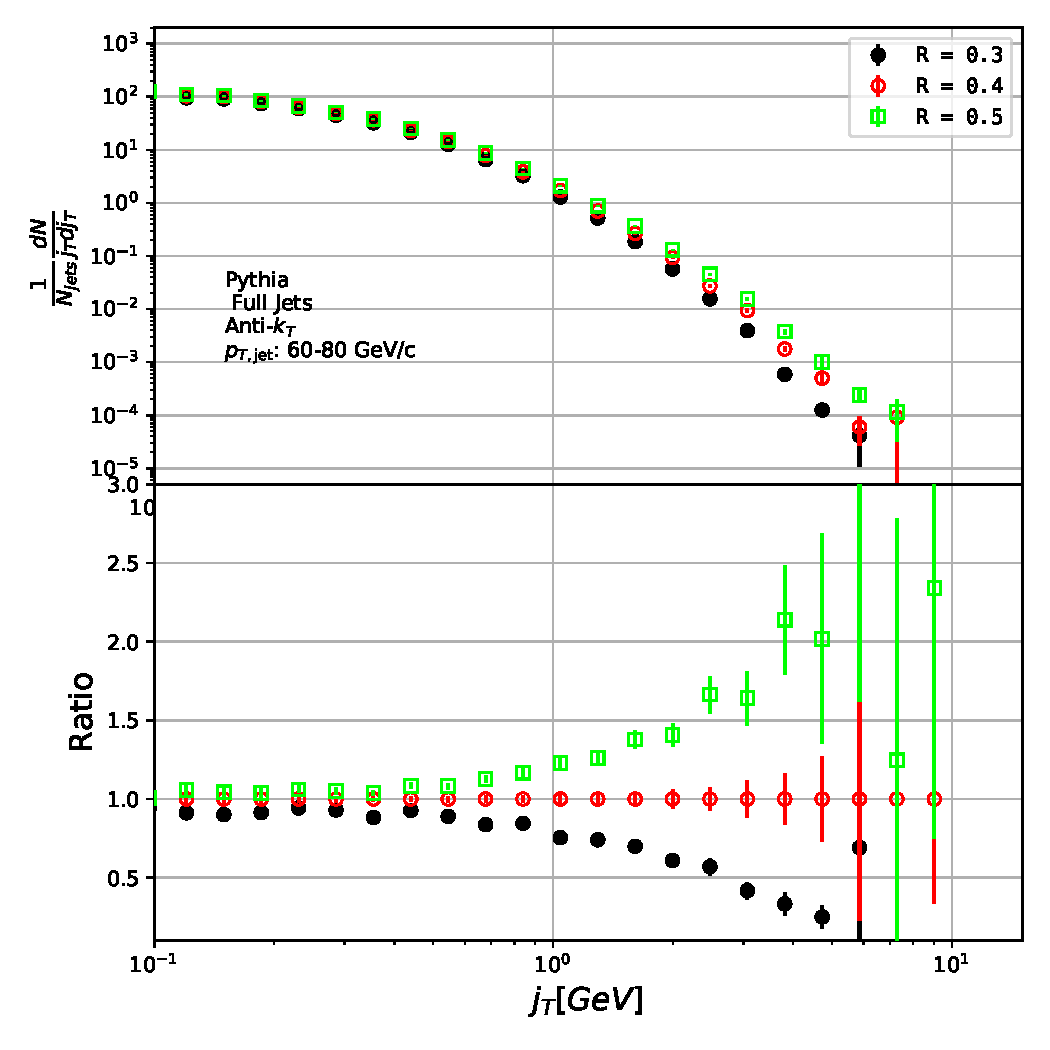
\includegraphics[width = 0.4\textwidth]{figures/results/RcomparisonSignalPt6080.pdf}}
\subfigure{ 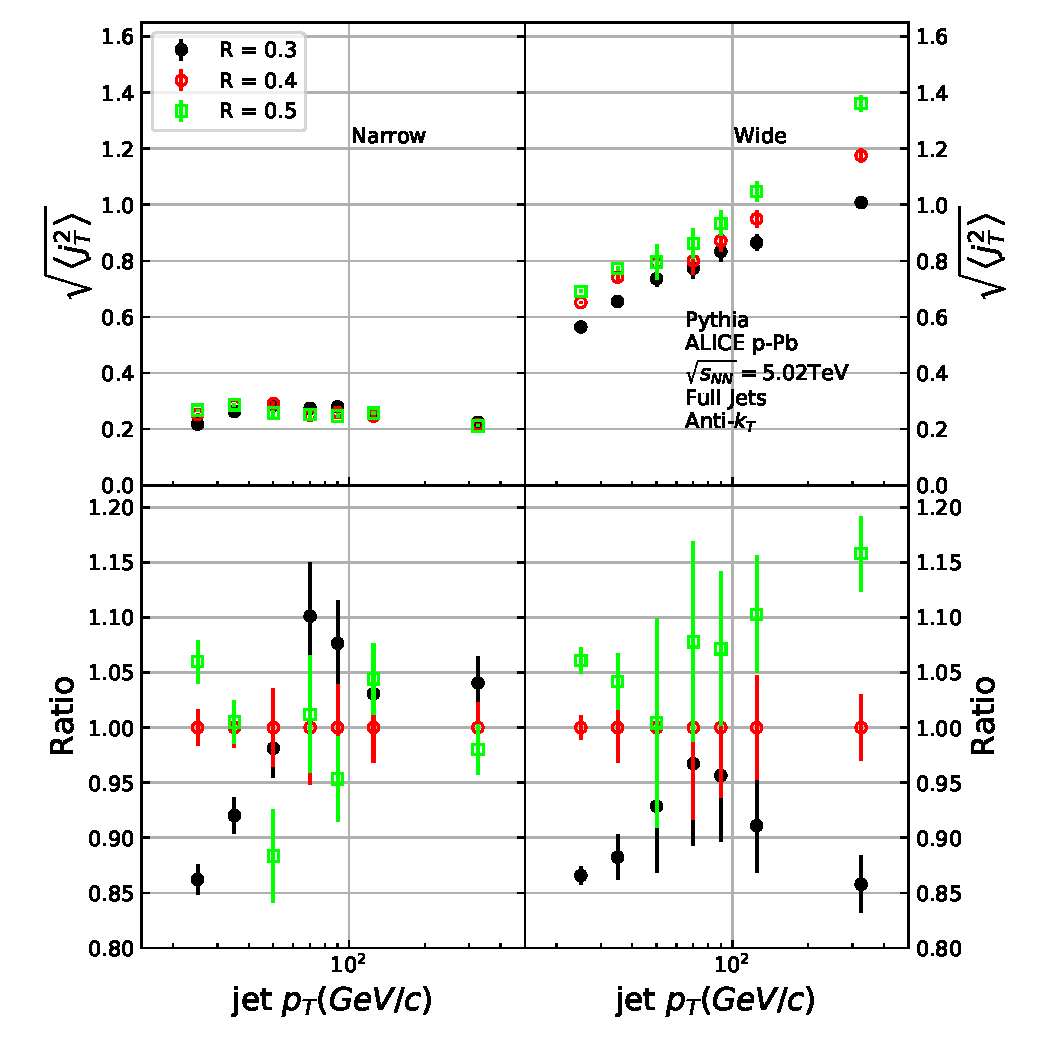
\includegraphics[width = 0.4\textwidth]{figures/results/RcomparisonRMS.pdf}}
\caption[\textsc{Pythia} $R$ parameters $\jt{}$]{Effect of changing $R$ parameter in jet finding on $\jt{}$ distributions}
\label{fig:Rcomparison}
\end{figure}


Effect of the $R$ parameter choice is studied in \textsc{Pythia}. Having a fixed cone puts hard limits on the possible $\jt{}$ values. Increasing the cone size loosens these limits and allows higher $\jt{}$ values. The results are shown in Fig. \ref{fig:Rcomparison}. Left hand side shows the $\jt{}$ distributions. There is very little change in low $\jt{}$ but at high $\jt{}$ the yield increases. 

This is also seen in the RMS values shown in the right hand side of Fig. \ref{fig:Rcomparison}, where the change in wide component RMS is about 10\% when going from $R=0.4$ to $R=0.3$ or $R=0.5$. With the narrow component values the situation is less clear. At low jet $\pt{}$ larger $R$ parameter leads to larger RMS values, but at hight $\pt{jet}$ the situation is reversed; increasing the $R$ parameter decreases RMS values.

Additionally the leading track is an imperfect estimate of the jet/original parton. Because the leading track in general is at an angle compared to the jet axis, the resulting $\jt{}$ values are different. In practice the jet axis found by the jet finding algrorithm tends to minimize the average $\jt{}$ of jet constituents. Thus the yield at high $\jt{}$ is limited and the RMS values are smaller.

A \textsc{Pythia} study was performed where $\jt{}$ was calculated with respect to the leading track momentum, instead of the jet axis. The results are shown in Fig. \ref{fig:RefComparison}. The resulting $\jt{}$ distributions are significantly wider than $\jt{}$ distributions from the typical method. The effect seems to be larger than the effect seen in comparing different $R$ values.

\begin{figure}[htp]
\centering
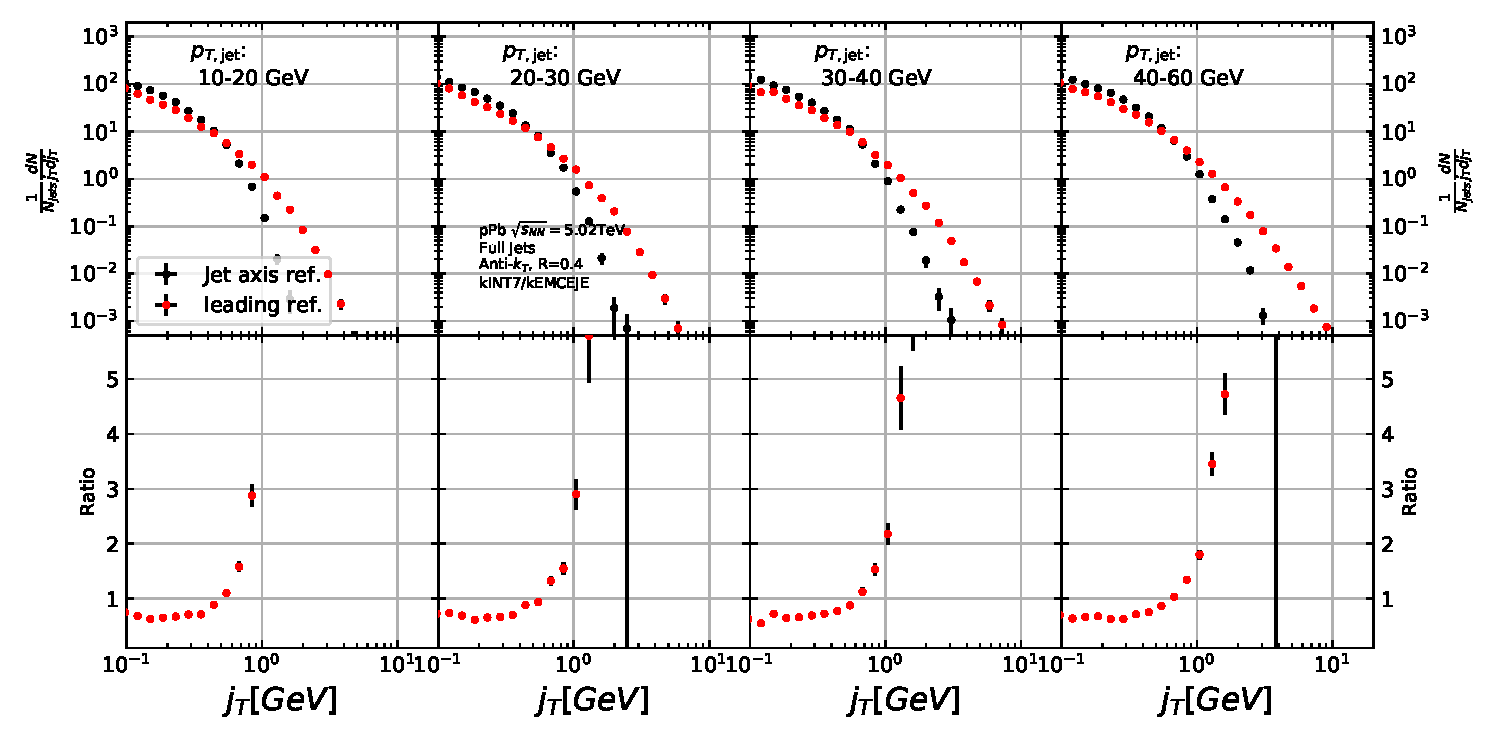
\includegraphics[width=0.55\textwidth]{figures/results/JetVsLeadingRefConst.pdf}
\caption{Results of calculating $\jt{}$ with respect to the jet axis or the leading hadron. The assumption is that because the leading hadron is an imperfect estimate of the jet axis, low $\jt{}$ tracks should on average be shifted to higher $\jt{}$}
\label{fig:RefComparison}
\end{figure}

\section{Conclusions}
\label{sec:conclusions}
In this work two distinct $\jt{}$ components were extracted for narrow and wide contributions using jet reconstruction. RMS values for both components were obtained. The width of the wide component is found to increase for increasing $\pt{jet}$. This is in part explained by the changing kinematical limits when going to higher $\pt{jet}$ which allows higher $\pt{track}$. Additionally the larger phase space allows stronger parton splitting. The results are qualitatively compatible with previous studies that studied $\jt{}$ using two-particle correlations.



 


%%%%% acknowledgements
\newenvironment{acknowledgement}{\relax}{\relax}
\begin{acknowledgement}
\section*{Acknowledgements}
%We wish to thank Torbjörn Sjöstrand for his help in defining a di-gluon initial state in \textsc{Pythia}~8.
%\input{acknowledgements.tex}    %%%%%%% done by webmaster team
\end{acknowledgement}

%%%%%%%% Bibliography (In case of using bibtex generate the bbl requested by arXiv)
\bibliographystyle{utphys}   % Remember we use title in the biblio
\bibliography{biblio}
%\input {bibliography.tex}  

%%%%%%%%% appendix with author list
\newpage
\appendix
%
%\input{}               %%%%%%%%%%% put your appendices here
%
\section{The ALICE Collaboration}
\label{app:collab}
%\input{authorlist-preprint.tex}  %%%%%%% done by webmaster team
\end{document}
